
%%%%%%%%%%%%%%%%%%%% author.tex %%%%%%%%%%%%%%%%%%%%%%%%%%%%%%%%%%%
%
% sample root file for your "contribution" to a contributed volume
%
% Use this file as a template for your own input.
%
%%%%%%%%%%%%%%%% Springer %%%%%%%%%%%%%%%%%%%%%%%%%%%%%%%%%%


% RECOMMENDED %%%%%%%%%%%%%%%%%%%%%%%%%%%%%%%%%%%%%%%%%%%%%%%%%%%
\documentclass[graybox]{svmult}

% choose options for [] as required from the list
% in the Reference Guide

\usepackage{type1cm}        % activate if the above 3 fonts are
                            % not available on your system
%
\usepackage{makeidx}         % allows index generation
\usepackage{graphicx}        % standard LaTeX graphics tool
                             % when including figure files
\usepackage{multicol}        % used for the two-column index
\usepackage[bottom]{footmisc}% places footnotes at page bottom


\usepackage{newtxtext}       % 
\usepackage{newtxmath}       % selects Times Roman as basic font

% see the list of further useful packages
% in the Reference Guide
\usepackage{latexsym}
\usepackage{multirow}
\usepackage{amsmath}
\usepackage{xcolor}


\makeindex             % used for the subject index
                       % please use the style svind.ist with
                       % your makeindex program

%%%%%%%%%%%%%%%%%%%%%%%%%%%%%%%%%%%%%%%%%%%%%%%%%%%%%%%%%%%%%%%%%%%%%%%%%%%%%%%%%%%%%%%%%

\begin{document}

\title*{An LSTM-based Approach for Insulin and Carbohydrate Recommendations in Type 1 Diabetes Self-Management}
%\title*{Towards Type 1 Diabetes Self-Management: Insulin and Carbohydrate Recommendations Using an LSTM-based Architecture}
%\title*{Automating Type 1 Diabetes Self-Management: Insulin and Carbohydrate Recommendations Using an LSTM-based Architecture}
\titlerunning{An LSTM-based Approach for Insulin and Carbohydrate Recommendations}
\author{Jeremy Beauchamp, Razvan Bunescu and Cindy Marling}
% Use \authorrunning{Short Title} for an abbreviated version of
% your contribution title if the original one is too long
\institute{Jeremy Beauchamp \at Ohio University, Athens, OH, \email{jb199113@ohio.edu}
  \and Razvan Bunescu \at University of North Carolina at Charlotte, Charlotte, NC \email{rbunescu@uncc.edu}
  \and Cindy Marling \at Ohio University, Athens, OH, \email{marling@ohio.edu}
}
%
% Use the package "url.sty" to avoid
% problems with special characters
% used in your e-mail or web address
%
\maketitle


\abstract{To avoid serious diabetic complications, people with type 1 diabetes must keep their blood glucose levels (BGLs) as close to normal as possible. Insulin dosages and carbohydrate consumption are important considerations in managing BGLs. Since the 1960s, models have been developed to forecast blood glucose levels based on the history of BGLs, insulin dosages, carbohydrate intake, and other physiological and lifestyle factors. Such predictions can be used to alert people to impending unsafe BGLs or to control insulin flow in an artificial pancreas. In past work, we have introduced an LSTM-based approach to blood glucose level prediction aimed at "what if" scenarios, in which people could enter foods they might eat or insulin amounts they might take and then see the effect on future BGLs.  Building on these neural models for "what-if" predictions, in this work we derive a novel LSTM-based architecture that can be trained to make either insulin or carbohydrate recommendations to ensure that future BGLs attain a desired level. Experimental evaluations using data from the OhioT1DM dataset show that the neural architecture substantially outperforms the baselines. The promising results suggest that this novel approach could potentially be of practical use to people with type 1 diabetes for self-management of BGLs.
%People with type 1 diabetes must constantly monitor their blood glucose levels and take actions to keep them from getting either too high or too low. Having a snack will raise blood glucose levels; however, the amount of carbohydrates that should be consumed to reach a target level depends on the recent history of blood glucose levels, meals, boluses, and the basal rate of insulin. Conversely, to lower the blood glucose level, one can administer a bolus of insulin; however, determining the right amount of insulin in the bolus can be cognitively demanding, as it depends on similar contextual factors. In this paper, we introduce a general LSTM-based architecture that can be trained to make either bolus or carbohydrate recommendations in order to get blood glucose to a desired level. Experimental evaluations using data from the OhioT1DM dataset show that the neural architecture substantially outperforms the baselines. The evaluations demonstrate that the proposed approach has a significant potential in reducing the cognitive burden imposed on people with type 1 diabetes.
}

\section{Introduction and Motivation}

%Type 1 diabetes is a disease in which the pancreas fails to produce insulin, which is required for blood sugar to be absorbed into cells. Without it, that blood sugar remains in the bloodstream, leading to high blood glucose levels (BGLs). In order to manage type 1 diabetes, insulin must be administered via an external source, such as injections or an insulin pump. People with type 1 diabetes also need to monitor their BGLs closely throughout the day by testing the blood acquired through finger-sticks and/or by using a continuous glucose monitoring (CGM) system. If the BGL gets too high (hyperglycemia) or too low (hypoglycemia), the individual responds by eating, taking insulin, or taking some other action to help get their BGL back to within a healthy range. An issue with this, however, is that the person with diabetes must \emph{react} to their BGL, whereas, ideally, they would be able to \emph{proactively} control their BGL. There has been much work in the area of BGL prediction in the past (\cite{bunescu:icmla13} and \cite{plis:maiha14} for example) with the aim of enabling preemptive actions to manage BGLs before individuals experience the negative symptoms of hypoglycemia or hyperglycemia. However, individuals still need to figure out how much to eat, how much insulin to take, and what other actions they can take to prevent hypoglycemia or hyperglycemia.

Diabetes self-management is a time-consuming, yet critical, task for people with type 1 diabetes.  To avoid serious diabetic complications, these individuals must continually manage their blood glucose levels (BGLs), keeping them as close to normal as possible.  They must avoid both low BGLs, or hypoglycemia, and high BGLs, or hyperglycemia, for their physical safety and well-being.  Diabetes self-management entails carefully monitoring BGLs throughout the day, by testing blood obtained from finger sticks and/or by using a continuous glucose monitoring (CGM) system.  It also entails making numerous daily decisions about the timing and dosage of insulin and the timing, ingredients, and quantity of food consumed.

Current diabetes self-management may be characterized as \emph{reactive}, rather than \emph{proactive}.  When BGLs are too high, individuals may take insulin to lower them, and when BGLs are too low, they may eat a snack or take glucose tablets to raise them.  The ability to accurately predict BGLs could enable people with type 1 diabetes to take preemptive actions \emph{before} experiencing the negative effects of hypoglycemia or hyperglycemia.  There have been efforts to model BGLs for the purpose of determining insulin dosages dating back to the 1960s \cite{boutayeb2016}.  There has been much recent work in BGL prediction for the purpose of providing support for diabetes self-management, including our own \cite{bunescu:icmla13,plis:maiha14}.  Accounts of some of the most recent BGL prediction efforts can be found in the proceedings of two international BGL prediction challenges \cite{kdh-2018-proceedings,kdh-2020-proceedings}.  It should be noted that, even with the benefit of accurate BGL predictions, individuals still need to determine how much to eat, how much insulin to take, and what other actions they can take to prevent hypoglycemia or hyperglycemia.

%The broad goal of the research presented in this paper is to essentially reverse the blood glucose prediction problem, and instead predict how many carbohydrates an individual should eat or how much insulin to administer with a bolus in order to get their BGL to the desired target. We have previously introduced in \cite{mirshekarian:embc19} an LSTM-based neural architecture that was trained such that it could answer {\it what-if} questions of the type “What will my BGL be in 60 minutes if I eat a snack with 30 carbs 10 minutes from now”. We show that by using the BGL target as a feature and the carbohydrates or insulin as labels, a similar architecture can be trained instead to predict the number of carbohydrates that need to be consumed or the amount of insulin that needs to be delivered during the prediction window in order to reach that BGL target.

The broad goal of the research presented here is to essentially reverse the BGL prediction problem, and instead predict how many grams of carbohydrate (carbs) an individual should eat or how much insulin they should take in order to achieve a desired BGL target. We have previously introduced an LSTM-based neural architecture that was trained to answer {\it what-if} questions of the type “What will my BGL be in 60 minutes if I eat a snack with 30 carbs 10 minutes from now?” \cite{mirshekarian:embc19}. We show that, by using the BGL target as a feature and the carbohydrates or insulin as labels, a similar architecture can be trained instead to predict the number of carbs that should be consumed or the amount of insulin that should be taken during the prediction window in order to reach that BGL target.

% This essentially is the next step after the future BGL is predicted, the patient then needs to take action to either correct or maintain their BGL. This system can help patients make sure that they are taking the appropriate action to accomplish this. This is implemented using recurrent neural networks on data gathered from Type 1 Diabetes patients.

The work by Mougiakakou and Nikita \cite{stavroula:dtt} represents one of the first attempts to use neural networks for recommending insulin regimens and dosages. Bolus calculators were introduced as early as 2003 \cite{zisser:dtt08}, wherein a standard formula is used to calculate the amount of bolus insulin based on parameters such as carbohydrate intake, carbohydrate-to-insulin ratio, insulin on board, and target BGL. Walsh et al. \cite{walsh:jdst18} discuss major sources of errors and potential ways to improve bolus advisors, such as utilizing the massive quantities of clinical data collected by the bolus advisors. As observed by Cappon et al.~in \cite{cappon:jdst18}, the standard formula approach ignores potentially useful preprandial conditions, such as the glucose rate of change. They propose a feed-forward fully connected neural network to exploit CGM information and some easily accessible patient parameters. Their experimental evaluations on simulated data show a small, but statistically significant, improvement in the blood glucose risk index. Simulated data is also used by Sun et al.~in \cite{sun:jbhi19}, where a basal-bolus advisor is trained using reinforcement learning in order to provide personalized suggestions to people with type 1 diabetes taking multiple daily injections of insulin.

The data-driven architecture introduced herein is generic in the sense that it can be trained to make recommendations about any variable that can impact BGLs, in particular, carbohydrates and insulin.  Carbohydrate recommendations are potentially useful when someone wants to prevent hypoglycemia well in advance or when someone wants to achieve a higher target BGL before physical exercise that is expected to lower it.  Bolus recommendations are useful prior to meals and also for lowering BGLs when individuals experience hyperglycemia. In \cite{beauchamp:kdh20}, we reported preliminary results only for the task of carbohydrate recommendation, where the aim was to achieve a desired target BGL 30 or 60 minutes into the future. The timing of the meal was variable within the prediction window and was used as one of the inputs to the model. In this paper, we change the task definition to make the system easier to use and more relevant to the type of situations encountered in the daily life of individuals with type 1 diabetes. As such, the timing of the bolus or meal is now fixed at 10 minutes into the future, based on the assumption that patients are most interested in using the system right before making a meal or bolus decision. To achieve the desired BGL, the user can specify any time horizon between 30 and 90 minutes, giving them more flexibility in terms of how fast they want their BGL to change. 

The rest of this chapter is organized as follows: Section 2 presents three different recommendation scenarios. Section 3 describes the neural architecture as well as the baselines used for comparison. Section 4 describes the dataset and explains how recommendation examples were derived. Section 5 explains the experimental methodology and presents the results of the experiments. Section 6 contains the conclusion and plans for future work.



\section{Three Recommendation Scenarios}

We assume that blood glucose levels are measured at 5 minute intervals through a CGM system. We also assume that discrete deliveries of insulin (boluses) and continuous infusions of insulin (basal rates) are recorded. Subjects provide the timing of meals and estimates of the number of grams of carbohydrate in each meal. Given the available data up to and including the present (time $t$), the system aims to estimate how much a person should eat or bolus 10 minutes from now (time $t+10$) such that their blood glucose will reach a target level $\tau$ minutes after that action (time $t + 10 + \tau$). A system that computes these estimates could then be used in the following three recommendation scenarios:
\begin{enumerate}
    \item {\bf Carbohydrate Recommendations}: Estimate the amount of carbohydrate $C_{t+10}$ to have in a meal in order to achieve a target BG value $G_{t+10+\tau}$.
    \item {\bf Bolus Recommendations}: Estimate the amount of insulin $B_{t+10}$ to deliver with a bolus in order to achieve a target BG value $G_{t+10+\tau}$.
    \item {\bf Bolus Recommendations given Carbohydrates}: Expecting that a meal with $C_{t+20}$ grams of carbohydrate will be consumed 20 minutes from now, estimate the amount of insulin $B_{t+10}$ to deliver with a bolus 10 minutes before the meal in order to achieve a target BG value $G_{t+10+\tau}$.
\end{enumerate}
These recommendation scenarios were designed to align with decision-making situations commonly encountered by people with type 1 diabetes. In particular, the corresponding recommendation systems would help an individual to estimate how much to eat or bolus for the purpose of raising or lowering their BGL (scenarios 1 and 2, respectively), as well as how much to bolus for a planned meal (scenario 3).

In the following section, we describe a number of baseline models and neural architectures using Long Short-Term Memory (LSTM) networks, all implementing the three types of recommendations. The LSTM-based models will be trained on examples extracted from the OhioT1DM dataset~\cite{ohiot1dm:marling:kdh18}, as explained in Section~\ref{sec:dataset}. Ideally, to match the intended use of these recommendations in practice, training examples should not have any extra meals or boluses in the prediction window $[t, t + 10 + \tau]$. Following the terminology from \cite{mirshekarian:embc19}, we call these examples {\it inertial}. However, to benefit from a larger number of training examples, we also train models on a more general class of {\it unrestricted} examples, in which other bolus or meal events are allowed to appear in the prediction window. In Section~\ref{sec:results} we show the extent to which models trained on the larger set of unrestricted examples transfer to inertial examples.

%Ideally, all examples of the above prediction scenarios in the data would not have any extra meals or boluses in the prediction window between $t$ and $t+10+\tau$. These events would not be known in practice since they are in the future. However, if only examples without these such events were used, it would limit the number of examples that can be extracted from the data. For this reason, examples are separated into 2 classes based on the following criteria:

%\begin{enumerate}
%    \item {\bf Class $\mathbf{C_{1}}$} examples do not contain events in the prediction window $(t, t+10+\tau)$ other than the meal or bolus that is to be predicted. When the bolus given carbohydrates prediction scenario is used, the meal that follows the bolus is also allowed in a C$_1$ example. This class of example most closely represents the situations in which the system would be used in practice. However, these examples are somewhat limited, especially for the bolus prediction scenario.
%    \item {\bf Class $\mathbf{C_{2}}$} is more general and allows other events to be in the prediction window $(t, t+10+\tau)$. This class yields a higher number of examples, but resembles a real world situation less than C$_1$, since there are unknown events past the present time $t$. Because of this, a more complex model is required to process C$_2$ examples.
%\end{enumerate}

%Using both classes of examples allows us to see how well the models do on examples similar to real world use, C$_1$, as well as how well the models do with the maximum number of possible examples in the dataset with C$_2$.

\section{Baseline Models and Neural Architectures}
\label{sec:models}

Given training data containing time series of blood glucose levels, meals with their carbohydrate intake, and boluses with their corresponding insulin dosages, we define the following two baselines:
\begin{enumerate}
    \item {\bf Global average}: 
    For the carbohydrate recommendation scenario, the average number $\mu$ of carbs over all of the meals in the subject's training data is computed and used as the estimate for all future predictions for that subject, irrespective of the context of the example. Analogously, for the bolus and bolus given carbs recommendation scenarios, $\mu$ is the average amount of insulin dosage over all boluses in the subject's training data. This is a fairly simple baseline, as it predicts the same average value for every test example for a particular subject.
    
    %Compute the average number of carbs over all of the meals in the subject's training data, and use this average $\mu$ as the estimate for all future meals, irrespective of context. This is a fairly simple baseline, as it predicts the same value for every example.
    \item {\bf ToD average}: In this Time-of-Day (ToD) dependent baseline, an average number of carbs or an average amount of bolus insulin is computed for each of the following five time windows during a day:
	\begin{itemize}
		\item 12am-6am: $\mu_1$ = early breakfast / late snacks.
		\item 6am-10am: $\mu_2$ = breakfast.
		\item 10am-2pm: $\mu_3$ = lunch.
		\item 2pm-6pm: $\mu_4$ = dinner.
		\item 6pm-12am: $\mu_5$ = late dinner / post-dinner snacks.
	\end{itemize}
    The average for each ToD interval is calculated over all of the meals or boluses appearing in the corresponding time frame in the subject's training data. At test time, to make a recommendation for time $t+10$, we first determine the ToD interval that contains $t+10$ and output the corresponding ToD average.
\end{enumerate}
Given sufficient historical data, the ToD baseline is expected to perform well for individuals who tend to eat very consistently and have regular diets. However, it is expected to perform poorly for individuals who have a lot of variation in their diets.

For the bolus given carbs recommendation scenario, one may ask why not also implement and evaluate a bolus calculator `baseline', for which insulin dosages would be computed using the actual bolus calculator employed by the subjects in the OhioT1DM dataset every time they had a meal. However, assuming subjects had perfect adherence to using the bolus calculator, this `baseline' would coincide with the ground truth every time, making it inappropriate as a baseline.

\begin{figure*}[t]
    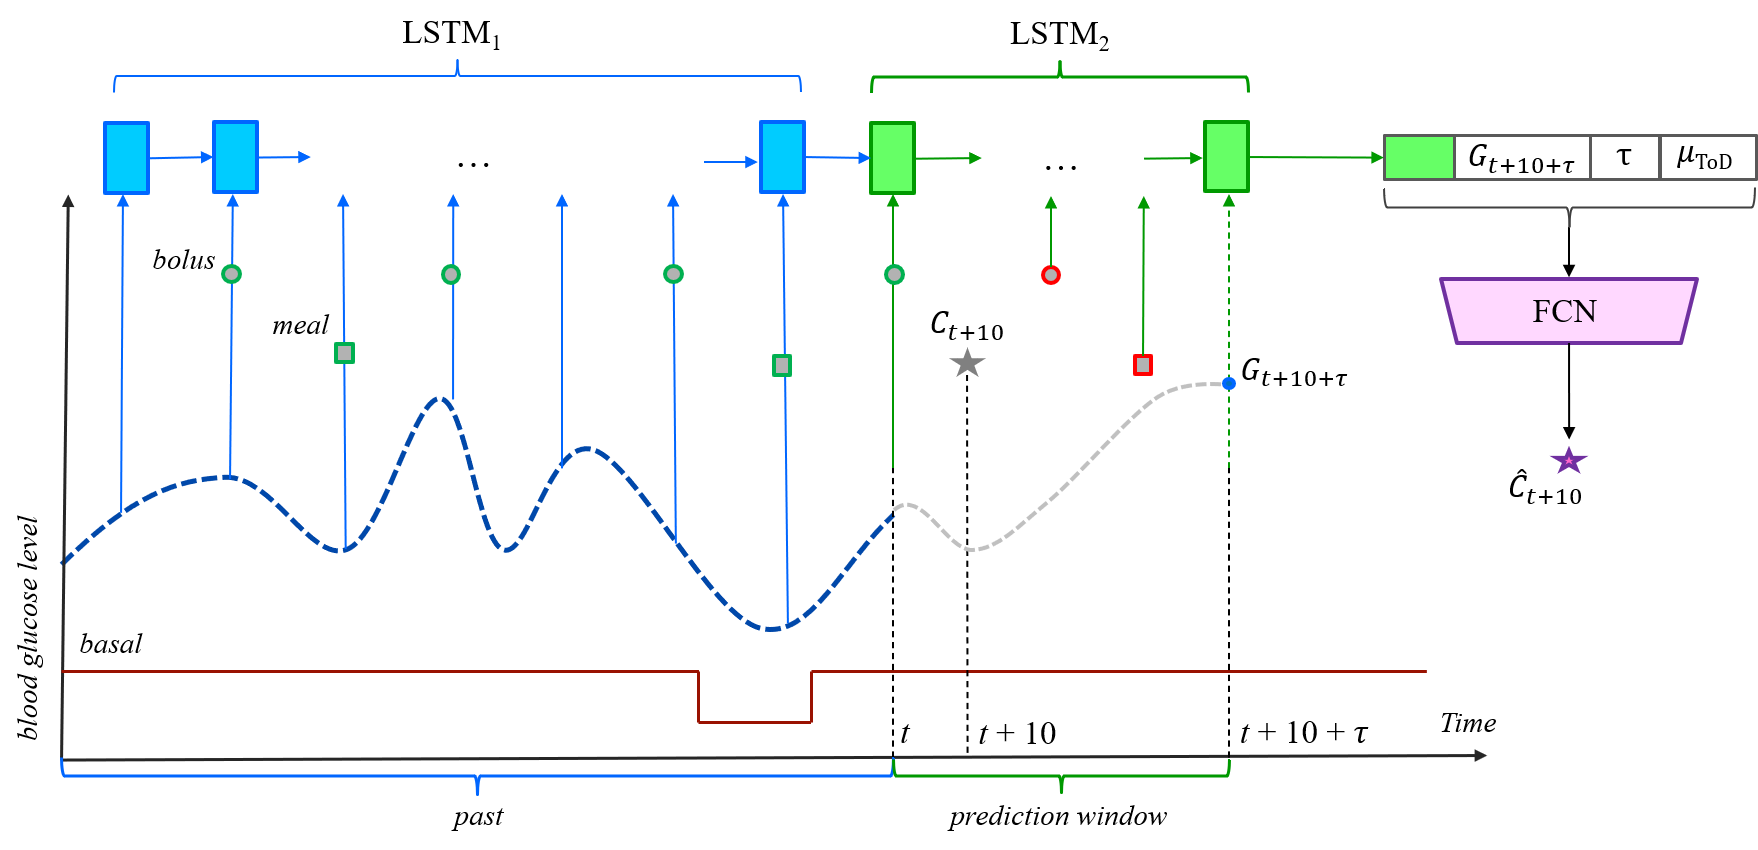
\includegraphics[width=\textwidth]{kdh_paper_diagram_1}
    \caption{The general neural network architecture for the carbohydrate recommendation scenario. The dashed blue line in the graph represents a subject's BGL, while the solid brown line represents the basal rate of insulin. The gray star represents the meal at $t+10$. The other meals are represented by squares, and boluses are represented by circles. Meals and boluses with a red outline cannot appear in {\it inertial} examples, but are allowed in {\it unrestricted} examples. The blue units in $\text{LSTM}_{1}$ receive input from different time steps in the past. The green units in $\text{LSTM}_{2}$ receive input from the prediction window. The purple trapezoid represents the 5 fully connected layers, whereas the output node at the end computes the prediction.}
    \label{fig:carbs}
\end{figure*}

\begin{figure*}[t]
    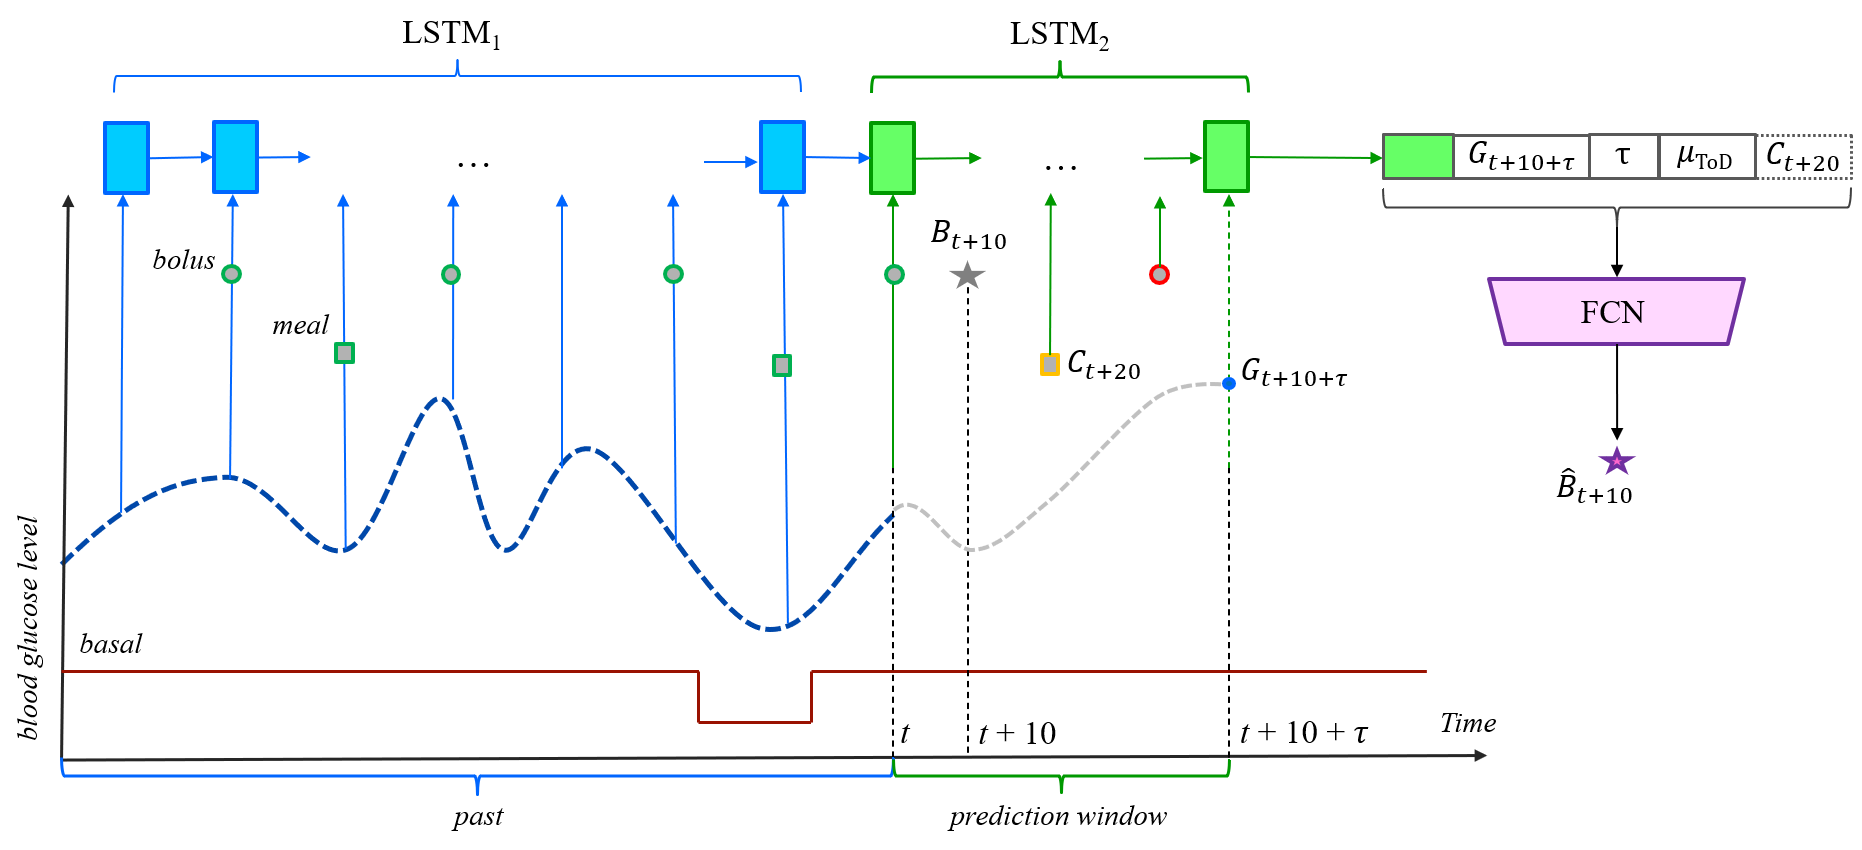
\includegraphics[width=\textwidth]{kdh_paper_diagram_2}
    \caption{The general neural network architecture for the bolus and bolus given carbs recommendation scenarios. The architecture itself is similar with that from Figure~\ref{fig:carbs}. The grey star now represents the bolus at $t+10$. For the bolus recommendation scenario, the events outlined in red or orange are not allowed in {\it inertial} examples.  However, in the bolus given carbs scenario, the meal event $C_{t+20}$ shown with the yellow outline is an important part of each example, be it inertial or unrestricted. As such, in this scenario, the dashed $C_{t+20}$ becomes part of the input to the FCN.}
    \label{fig:bolus}
\end{figure*}

While simple to compute and use at test time, the two baselines are likely to give suboptimal performance, as their predictions ignore the history of BGL values, insulin (boluses and basal rates), and meals, all of which could significantly modulate the effect a future meal and/or bolus might have on the BGL. To exploit this information, we use the general LSTM-based network architecture shown in Figure~\ref{fig:carbs}. The first component in the architecture is a recurrent neural network instantiated using Long Short-Term Memory (LSTM) cells \cite{hochreiter:nc97}, which is run over the previous 6 hours of data, up to and including the present time $t$. At each time step (every 5 minutes), this LSTM$_1$ network takes as input the BGL, the carbs, and the insulin dosages recorded at that time step. While sufficient for processing {\it inertial} examples, this LSTM cannot be used to process events that may appear in the prediction window $(t, t+10+\tau)$ of {\it unrestricted} examples, because BGL values are not available in the future. Therefore, when training on unrestricted examples, the final state computed by the LSTM$_1$ model at time $t$ is projected using a linear transformation and used as the initial state for a second LSTM model, LSTM$_2$, that is run over all the time steps in the prediction window $(t, t+10+\tau)$. The final state computed either by LSTM$_1$ (for intertial examples) or LSTM$_2$ (for unrestricted examples) is then used as input to a fully connected network (FCN) whose output node computes an estimate of the carbs or bolus insulin at time $t+10$. In addition to the LSTM final state, the input to the FCN contains the following features:
\begin{itemize}
    \item The target blood glucose level $\tau+10$ minutes into the future, i.e., $G_{t + 10 + \tau}$.
    \item The prediction horizon $\tau$.
    \item The ToD average for the time frame that contains $t+10$.
    \item For the bolus given carbs scenario only, the planned amount $C_{t + 20}$ of carbohydrate becomes part of the input, too.
\end{itemize}
Each LSTM uses vectors of size 32 for the states and gates, whereas the FCN is built with 5 hidden layers, each consisting of 64 ReLU neurons, and one linear output node.

\section{Using the OhioT1DM Dataset for Recommendation Examples}
\label{sec:dataset}

To evaluate the proposed recommendation models, we create training and test examples based on data collected from 6 subjects with type 1 diabetes that is distributed with the OhioT1DM dataset~\cite{ohiot1dm:marling:kdh20}. Time series containing the basal rate of insulin, boluses, meals, and BGL readings were collected over roughly 50 days, although the exact number of days varies from subject to subject. 
Insulin and BGL data was automatically recorded by each subject's insulin pump.  Meal data was collected in two different ways.  Subjects self reported meal times and estimated carbs via a smartphone interface.  Subjects also entered estimated carbs into a "Bolus Wizard," or calculator, when bolusing for meals, and this data was recorded by the insulin pump.

While exploring the data, it was observed that self-reported meals and their associated boluses were in unexpected temporal positions relative to each other. For many meals, patients recorded a timestamp in the smartphone interface that preceded the corresponding bolus timestamp recorded in the insulin pump. This was contrary to what was recommended to the subjects by their physicians, which was to bolus shortly before the meal, and no more than 15 minutes prior to the meal. This discrepancy is likely due to subjects reporting incorrect meal times in the smartphone interface.

{\bf Pre-processing of meals}: To correct the meal events, we used the data input to the Bolus Wizard in the insulin pump and ran a pre-processing step that changed the timestamp of each meal associated with a bolus to be exactly 10 minutes after that bolus. For these meals, we also used the number of carbs provided to the Bolus Wizard, which is likely to be more accurate than the estimate provided by the subject through the smartphone interface. To determine the meal event that is associated with a bolus having non-zero carb input, we searched for the meal that was closest in time to the bolus, either before or after. In case there are 2 meals that are equally close to the bolus, we selected the one for which the number of carbs from the smartphone interface is closest to the number of carbs entered into the Bolus Wizard. Experimental results reported in Section~\ref{sec:results} show that this pre-processing of meal events leads to significantly more accurate predictions, which indirectly justifies the pre-processing.

Table \ref{tab:meals} shows the number of meals in each subject's pre-processed data, together with statistics such as the minimum, maximum, median, average, and standard deviation for the number of carbs per meal. Table~\ref{tab:boluses} shows the same statistics for boluses and their dosages, expressed in units of insulin.
\begin{table}[h]\setlength{\tabcolsep}{4pt}
\begin{center}
\caption{Per subject and total meal and carbohydrate statistics: Minimum, Maximum, Median, Average, and Standard Deviation (StdDev).}
\label{tab:meals}
\begin{tabular}{|cr|rrrrc|}
    \cline{3-7}
    \multicolumn{2}{c}{} & \multicolumn{5}{|c|}{Carbs Per Meal}\\
	\hline
	Subject & \multicolumn{1}{c|}{Meals} & \multicolumn{1}{c}{Minimum} & \multicolumn{1}{c}{Maximum}
	& \multicolumn{1}{c}{Median} & \multicolumn{1}{c}{Average} & StdDev\\
	\hline
	559 & 179 & 8.0 & 75.0 & 30.0 & 34.6 & 15.1\\
    563 & 153 & 5.0 & 84.0 & 34.0 & 35.6 & 18.4\\
    570 & 169 & 5.0 & 200.0 & 115.0 & 106.3 & 41.6\\
	575 & 284 & 2.0 & 110.0 & 40.0 & 40.2 & 21.9\\
	588 & 257 & 2.0 & 60.0 & 20.0 & 22.4 & 14.6\\
	591 & 248 & 3.0 & 77.0 & 28.0 & 31.4 & 14.1\\
	\hline
	Total & 1290 & 2.0 & 200.0 & 34.0 & 42.3 & 33.7\\
	\hline
\end{tabular}
\end{center}
\end{table}
\begin{table}[h]\setlength{\tabcolsep}{4pt}
\begin{center}
\caption{Per subject and total boluses and insulin units statistics: Minimum, Maximum, Median, Average, and Standard Deviation (StdDev).}
\label{tab:boluses}
\begin{tabular}{|cr|rrrrc|}
    \cline{3-7}
    \multicolumn{2}{c}{} & \multicolumn{5}{|c|}{Insulin Per Bolus}\\
	\hline
	Subject & \multicolumn{1}{c|}{Boluses}
	& \multicolumn{1}{c}{Minimum} & \multicolumn{1}{c}{Maximum} & \multicolumn{1}{c}{Median} & \multicolumn{1}{c}{Average} & StdDev\\
	\hline
	559 & 186 & 0.1 & 9.3 & 3.6 & 3.7 & 1.9\\
    563 & 424 & 0.1 & 24.7 & 7.8 & 8.0 & 4.2\\
    570 & 1,345 & 0.2 & 12.1 & 1.3 & 1.8 & 2.1\\
	575 & 271 & 0.1 & 12.8 & 4.4 & 4.1 & 3.0\\
	588 & 221 & 0.4 & 10.0 & 3.5 & 4.3 & 2.3\\
	591 & 331 & 0.1 & 9.4 & 2.9 & 3.1 & 1.8\\
	\hline
	Total & 2758 & 0.1 & 24.7 & 1.9 & 3.5 & 3.4\\
	\hline
\end{tabular}
\end{center}
\end{table}
The numbers in Table~\ref{tab:meals} show that most subjects have a similar average number of carbs in their meals, with the exception of 570 who has a significantly larger number of carbs per meal on average. More importantly, subject 570 also has a much higher standard deviation than the other subjects, which is likely to make the recommendation task more difficult in their case.

The number of boluses varies from subject to subject more so than the number of meals. Most subjects had similar average and standard deviations, with the exception of subject 563, who had a much larger average and standard deviation than the rest of the subjects. It is also interesting to note that subject 570 had a lower bolus average than most subjects and far more boluses than any of the others. Subject 570 used many dual boluses, which we did not include as prediction labels, since the scope of the project to date supports only recommendations for regular boluses.


\subsection{From Meals and Bolus Events to Recommendation Examples}
\label{sec:examples}

In all recommendation scenarios, the prediction window ranges between the present time $t$ and the prediction horizon $t + 10 + \tau$. For the carbohydrate or bolus recommendation scenarios, the meal or the bolus is assumed to occur at time $t +10$. For the bolus given carbs scenario, the bolus occurs at time $t+10$ and is followed by a meal at time $t+20$, which matches the pre-processing of the meal data. For evaluation purposes, we set $\tau$ to values between 30 and 90 minutes with a step of 5 minutes, i.e, $\tau \in \{30, 35, 40, ..., 90\}$ for a total of 13 different values. As such, each meal/bolus event in the data results in 13 recommendation examples, one example for each value of $\tau$. While all 13 examples use the same value for the prediction label, e.g., $B_{t + 10}$ for bolus prediction, they will differ in terms of the target BG feature $G_{t + 10 + \tau}$ and the $\tau$ feature, both used directly as input to the FCN module in the architectures shown in Figures~\ref{fig:carbs} and~\ref{fig:bolus}. For the bolus given carbs scenario, the 13 examples are only created when there is a meal that had a bolus delivered 10 minutes prior. Due to the way the data is pre-processed, it is guaranteed that if a meal had a bolus associated with it, the bolus will be exactly 10 minutes before the meal. 

Table \ref{tab:c1_examples} shows the number of {\it inertial} examples for 5 prediction horizons, as well as the total over all 13 possible prediction horizons. Table \ref{tab:c2_examples} shows the number of {\it unrestricted} examples. Since the same number of {\it unrestricted}  examples are available for every prediction horizon, only the totals are shown. The only exceptions would be if an event was near the end of a subject's data and the prediction horizon $t+10+\tau$ goes past the end of the dataset for some value of $\tau$.

\begin{table*}\setlength{\tabcolsep}{4pt}
\begin{center}
\caption{{\it Inertial} ({\it I}) examples by recommendation scenario and prediction horizon.}
\label{tab:c1_examples}
\begin{tabular}{|l|rrrr|}

    \hline
    \multicolumn{5}{|c|}{Carbohydrate recommendation}\\
    \hline
    Horizon & Training & Validation & Testing & Total {\it I}\\
    \hline
%    \multirow{6}{*}{Carbohydrate}
    $\tau=30$ & 700 & 190 & 168 & 1,058\\
    $\tau=45$ & 684 & 188 & 165 & 1,037\\ 
    $\tau=60$ & 664 & 181 & 163 & 1,008\\
    $\tau=75$ & 632 & 177 & 155 & 964\\ 
    $\tau=90$ & 597 & 170 & 150 & 917\\
    All 13 horizons & 8,546 & 2,356 & 2,088 & 12,990\\
    \hline
    \hline
    \multicolumn{5}{|c|}{Bolus recommendation}\\
    \hline
%    \multirow{6}{*}{Bolus}
    Horizon & Training & Validation & Testing & Total {\it I}\\
    \hline
    $\tau=30$ & 345 & 91 & 107 & 543\\
    $\tau=45$ & 324 & 88 & 101 & 513\\ 
    $\tau=60$ & 293 & 82 & 89 & 464\\
    $\tau=75$ & 258 & 76 & 81 & 415\\ 
    $\tau=90$ & 234 & 67 & 72 & 373\\
    All 13 horizons & 3,790 & 1,054 & 1,176 & 6,020\\
    \hline
    \hline
%    \multirow{6}{*}{Bolus Given Carbs}
    \multicolumn{5}{|c|}{Bolus given carbs recommendation}\\
    \hline
    Horizon & Training & Validation & Testing & Total {\it I}\\
    \hline
    $\tau=30$ & 488 & 143 & 142 & 773\\
    $\tau=45$ & 483 & 142 & 140 & 765\\ 
    $\tau=60$ & 474 & 139 & 139 & 752\\
    $\tau=75$ & 460 & 134 & 136 & 730\\ 
    $\tau=90$ & 444 & 133 & 130 & 707\\
    All 13 horizons & 6,118 & 1,799 & 1,789 & 9,706\\
    \hline
    
\end{tabular}
\end{center}
\end{table*}

\begin{table*}\setlength{\tabcolsep}{4pt}
\begin{center}
\caption{{\it Unrestricted} (U) examples by recommendation scenario. Also showing in the last column the total number of non-inertial ($U - I$) examples.}
\label{tab:c2_examples}
\begin{tabular}{|l|rrrr|r|}
	\hline
	Recommendation scenario & Training & Validation & Testing & Total $U$ & Total $U - I$\\
	\hline
	Carbohydrate & 10,899 & 2,964 & 2,665 & 16,528 & 3,538\\
	Bolus & 12,282 & 3,595 & 3,810 & 19,687 & 13,667\\
	Bolus given carbs & 7,407 & 2,236 & 2,276 & 11,919 & 2,213\\
	\hline
\end{tabular}
\end{center}
\end{table*}

For the carbohydrate and bolus given carbs recommendation scenarios, the gap between the number of {\it inertial} and {\it unrestricted} examples is not very large, as most examples qualify as inertial examples. However, in the bolus recommendation scenario, there is a very sizable gap between the number of inertial vs. unrestricted examples. This is because a significant number of boluses are associated with meals, and since these meals are timestamped to be 10 minutes after the bolus, the result is that a bolus at time $t + 10$ will be associated with a meal at time $t + 20$. Therefore, for preprandial boluses at $t + 10$, the meal at time $t + 20$ will prohibit the creation of inertial recommendation examples, because by definition inertial examples do not allow the presence of other events in the prediction window $(t, t + 10 + \tau)$.
% every bolus that had a meal associated with it will have been taken 10 minutes prior to a meal. This means there is a meal at $t+20$ for every bolus that was associated with a meal. This meal will disallow an example to be classified as a C$_1$ example since $t+20$ is within the prediction window. This same effect does not apply for the bolus given carbohydrates prediction scenario is because the meal at $t+20$ is allowed in C$_1$ examples in this scenario. If this were not the case, there would be zero C$_1$ examples for the bolus given carbohydrates prediction scenario.

\section{Experimental Methodology and Results}
\label{sec:evaluation}

For each of the 6 subjects in the dataset, their time series data is split into three sets, as follows:
\begin{itemize}
    \item {\it Testing}: the last 10 days of data.
    \item {\it Validation}: the 10 days of data preceding the testing portion.
    \item {\it Training}: the remainder of the data, around 30 days.
\end{itemize}
The blood glucose, carbs, and insulin values are all scaled to be between $[0, 1]$ by using maximum and minimum values computed over training data. When computing the performance metrics at test time, the predicted values are scaled back to the original range.
The neural architecture is trained to minimize the mean squared error between the actual event (meal or bolus) value recorded in the training data and the estimated value computed by the output node of the FCN module. The Adam \cite{kingma:adam} variant of gradient descent is used for training, with the learning rate and mini-batch size being tuned on the validation data. In an effort to avoid overfitting, early stopping with a patience of 10 epochs and dropout with a rate of 10\% are used in all experiments.

Before training a personalized model for a specific subject, a generic model is first pre-trained on the union of all 6 subjects' training data. The generic model is then fine tuned separately for each individual subject, by continuing training on that subject's training data only. The pre-training allows the model parameters to be in a better starting position before fine tuning, allowing faster and better training. The learning rate and batch size are tuned for each subject on their validation data. Once the hyper-parameters are tuned, the final models are then fine tuned on the union of the training and validation data for each subject for a maximum of 100 epochs. For each subject, the results are aggregated over 5 models that are trained with different seedings of the random number generators.

The metrics used to evaluate the models are the Root Mean Squared Error (RMSE) and the Mean Absolute Error (MAE). Two scores are reported for each evaluation of the LSTM-based recommendation model:
\begin{enumerate}
    \item The {\bf Model.mean} score calculates the average RMSE and MAE on the testing data across the 5 models trained for each subject, and then averages these scores across all 6 subjects.
    \item The {\bf Model.best} score instead selects for each subject the model that performed best in terms of MAE on the validation data, out of the 5 models trained for that subject. The RMSE and MAE test scores are averaged over all 6 subjects.
\end{enumerate}
Two sets of LSTM-based models were trained for each of the three recommendation scenarios: a set of models were trained and evaluated on {\it inertial} examples and a set was trained and evaluated on {\it unrestricted} examples. For the carbohydrate and bolus given carbs scenarios, there were no inertial examples in subject 570's testing data. To make the results comparable, subject 570 is not used for computing the results in these scenarios.

\subsection{Experimental Results}
\label{sec:results}

\begin{table*}[t]\setlength{\tabcolsep}{4pt}
\caption{Results for each recommendation scenario, for both classes of examples.}
\begin{center}
\label{tab:results}
\begin{tabular}{|l|rr|rr|}

   	\cline{2-5}
	\multicolumn{1}{c}{} & \multicolumn{2}{|c|}{Inertial} & \multicolumn{2}{c|}{Unrestricted}\\
	\hline
	Carbohydrate recommendation & RMSE & MAE & RMSE & MAE\\
	\hline
	Global Average & 16.58 & 13.66 & 16.54 & 13.65\\
	ToD Average & 15.91 & 12.92 & 15.96 & 12.97\\
	\hline
	Model.mean & \textbf{9.61} & 7.32 & \textbf{9.37} & \textbf{7.00}\\
	Model.best & 9.68 & \textbf{7.09} & 9.88 & 7.24\\
	\hline
	\multicolumn{5}{c}{}\\[-1.5ex]
   	\cline{2-5}
	\multicolumn{1}{c}{} & \multicolumn{2}{|c|}{Inertial} & \multicolumn{2}{c|}{Unrestricted}\\
	\hline
	Bolus recommendation & RMSE & MAE & RMSE & MAE\\
	\hline
	Global Average & 2.19 & 1.87 & 3.05 & 2.51\\
	ToD Average & 2.28 & 1.82 & 2.97 & 2.38\\
	\hline
	Model.mean & \textbf{1.64} & 1.22 & \textbf{1.54} & \textbf{1.14}\\
	Model.best & \textbf{1.64} & \textbf{1.20} & 1.58 & 1.17\\
	\hline
	\multicolumn{5}{c}{}\\[-1.5ex]
   	\cline{2-5}
	\multicolumn{1}{c}{} & \multicolumn{2}{|c|}{Inertial} & \multicolumn{2}{c|}{Unrestricted}\\
	\hline
	Bolus given carbs recommendation & RMSE & MAE & RMSE & MAE\\
	\hline
	Global Average & 2.64 & 2.23 & 2.67 & 2.25\\
	ToD Average & 2.55 & 2.08 & 2.56 & 2.10\\
	\hline
	Model.mean & 1.18 & 0.93 & 1.10 & 0.81\\
	Model.best & \textbf{1.17} & \textbf{0.89} & \textbf{1.06} & \textbf{0.77}\\
	\hline
\end{tabular}
\end{center}
\end{table*}


Table~\ref{tab:results} shows the results for the two baselines and the LSTM-based models. Across all scenarios and for both example classes, the neural models outperform both baselines by a wide margin.  There also is very little difference between the best model scores and the average model scores, which means that the model performance is stable with respect to the random initialization of the network parameters.

\begin{table*}\setlength{\tabcolsep}{4pt}
\caption{Comparison between models trained on Inertial vs. Unrestricted examples, in terms of their performance on Inertial examples.}
\begin{center}
\label{tab:transfer}
\begin{tabular}{|l|l|l|c|c|}
	
    \cline{3-5}
    \multicolumn{2}{c|}{} & Trained on & RMSE & MAE\\
    \hline
    \multirow{4}{*}{Carbohydrate recommendation} & \multirow{2}{*}{Model.mean} & Inertial & 9.61 & 7.32\\
    & & Unrestricted & \textbf{9.35} & \textbf{7.01}\\
    \cline{2-5}
    & \multirow{2}{*}{Model.best} & Inertial & 9.68 & 7.09\\
    & & Unrestricted & 9.70 & 7.13\\
    \hline
    
    \multirow{4}{*}{Bolus recommendation} & \multirow{2}{*}{Model.mean} & Inertial & \textbf{1.64} & \textbf{1.22}\\
	& & Unrestricted & 1.77 & 1.38\\
   \cline{2-5}
    & \multirow{2}{*}{Model.best} & Inertial & \textbf{1.64} & \textbf{1.20}\\
    & & Unrestricted & 1.85 & 1.46\\
    \hline
    
    \multirow{4}{*}{Bolus given carbs recommendation} & \multirow{2}{*}{Model.mean} & Inertial & 1.18 & 0.93\\
    & & Unrestricted & \textbf{1.10} & \textbf{0.82}\\
	
   \cline{2-5}
    & \multirow{2}{*}{Model.best} & Inertial & 1.17 & 0.89\\ 
    & & Unrestricted & \textbf{1.07} & \textbf{0.78}\\
    \hline

\end{tabular}
\end{center}
\end{table*}

Of the results reported in Table~\ref{tab:results}, the most relevant for practical scenarios are the evaluations on inertial examples; unrestricted examples subsume examples that contain information about future events, which is difficult to have in practice. However, the set of unrestricted examples is larger; as such, it has the potential to improve performance on inertial examples through transfer learning. To determine if and to what extent transfer happens, in Table~\ref{tab:transfer} we compare LSTM-based models trained on {\it inertial} vs. {\it unrestricted} examples, in terms of their performance on inertial examples. For the carbohydrate and bolus given carbs recommendation scenarios, the results show that training on the extra non-inertial examples provided by the unrestricted dataset help achieve better performance on the inertial examples. However, this type of positive transfer does not happen in the bolus recommendation scenario, for which the models trained solely on inertial examples performed better. This can be explained by the fact that there are two types of bolus events: boluses associated with meals, which are intended to {\it proactively} prevent spikes in blood glucose due to carbs in the meals, and boluses that are administered {\it reactively} to lower already high blood glucose levels. The bolus recommendation entry in the last column of Table~\ref{tab:c2_examples} shows that the pre-prandial, proactive bolus examples represent the vast majority of unrestricted bolus examples: i.e., 13,667 out of 19,687, which is more than twice the 6,020 inertial, reactive bolus examples shown in Table~\ref{tab:c1_examples}. As such, a bolus recommendation model that is trained on unrestricted bolus examples is likely to be biased towards pre-prandial boluses for which the blood glucose behavior is different compared with the inertial, reactive boluses on which the model is evaluated.

In all experiments reported so far, one model was trained for all prediction horizons, using the value of $\tau \in \{30, 35, ..., 90\}$ as an additional input feature for the FCN component. This global mode was then tested on examples from all prediction horizons. To determine if transfer learning also happens among different prediction horizons, for each value of $\tau \in \{30, 45, 60, 75, 90\}$ at test time, we compare the performance of the globally trained model vs. the performance of a model trained only on examples for that particular prediction horizon, using unrestricted examples for both. The results in Table \ref{tab:time_transfer} show transfer learning clearly happening for the carbohydrate and bolus recommendation scenarios, where the models trained on all prediction horizons outperform those trained only on a specific prediction horizon when evaluated on that prediction horizon. For the bolus given carbs prediction scenario, the results are roughly the same.


\begin{table*}\setlength{\tabcolsep}{1.75pt}
\caption{Comparison between models trained on all prediction horizons vs. one prediction horizon $\tau$, when evaluated on the prediction horizon $\tau$.}
\begin{center}
\label{tab:time_transfer}
\begin{tabular}{|c|c|rr|rr|rr|rr|rr|rr|rr}
    \cline{3-14}
    \multicolumn{2}{c|}{} & \multicolumn{12}{c|}{Carbohydrate recommendation}\\
    \cline{3-14}
    \multicolumn{2}{c|}{} & \multicolumn{2}{c|}{$\tau=30$} & \multicolumn{2}{c|}{$\tau=45$} & \multicolumn{2}{c|}{$\tau=60$} & \multicolumn{2}{c|}{$\tau=75$} & \multicolumn{2}{c|}{$\tau=90$} & \multicolumn{2}{c|}{Average}\\
    \cline{2-14}
     \multicolumn{1}{c|}{}& Trained on & \multicolumn{2}{c|}{\scriptsize RMSE MAE} & \multicolumn{2}{c|}{\scriptsize RMSE MAE} & \multicolumn{2}{c|}{\scriptsize RMSE MAE} & \multicolumn{2}{c|}{\scriptsize RMSE MAE} & \multicolumn{2}{c|}{\scriptsize RMSE MAE} & \multicolumn{2}{c|}{\scriptsize RMSE MAE} \\
    \hline
    \multirow{2}{*}{Model.mean} & One $\tau$ & 11.43 & 8.40 & 12.04 & 8.96 & 11.69 & 8.57 & 11.90 & 9.01 & 11.96 & 9.25 & 11.80 & 8.84\\
    & All $\tau$ & \textbf{10.79} & \textbf{8.08} & \textbf{10.56} & \textbf{7.77} & \textbf{10.44} & \textbf{7.69} & \textbf{10.84} & \textbf{7.96} & \textbf{10.69} & \textbf{7.93} & \textbf{10.66} & \textbf{7.89}\\
    \hline
    \multirow{2}{*}{Model.best} & One $\tau$ & 11.17 & 8.34 & 11.83 & 8.57 & 11.46 & 8.28 & 11.77 & 8.63 & 11.58 & 8.80 & 11.56 & 8.52\\
    & All $\tau$ & \textbf{10.87} & \textbf{8.15} & \textbf{10.79} & \textbf{7.75} & \textbf{10.44} & \textbf{7.54} & \textbf{10.71} & \textbf{7.83} & \textbf{10.66} & \textbf{7.84} & \textbf{10.69} & \textbf{7.82}\\
    \hline
    
    \multicolumn{14}{c}{}\\[-1.5ex]

    \cline{3-14}
    \multicolumn{2}{c|}{} & \multicolumn{12}{c|}{Bolus recommendation}\\
    \cline{3-14}
    \multicolumn{2}{c|}{} & \multicolumn{2}{c|}{$\tau=30$} & \multicolumn{2}{c|}{$\tau=45$} & \multicolumn{2}{c|}{$\tau=60$} & \multicolumn{2}{c|}{$\tau=75$} & \multicolumn{2}{c|}{$\tau=90$} & \multicolumn{2}{c|}{Average}\\
    \cline{2-14}
     \multicolumn{1}{c|}{}& Trained on & \multicolumn{2}{c|}{\scriptsize RMSE MAE} & \multicolumn{2}{c|}{\scriptsize RMSE MAE} & \multicolumn{2}{c|}{\scriptsize RMSE MAE} & \multicolumn{2}{c|}{\scriptsize RMSE MAE} & \multicolumn{2}{c|}{\scriptsize RMSE MAE} & \multicolumn{2}{c|}{\scriptsize RMSE MAE} \\
    \hline
    \multirow{2}{*}{Model.mean} & One $\tau$ & 1.70 & 1.21 & 1.65 & 1.18 & 1.58 & 1.18 & 1.59 & 1.17 & 1.64 & 1.20 & 1.63 & 1.19\\
    & All $\tau$ & \textbf{1.53} & \textbf{1.11} & \textbf{1.49} & \textbf{1.10} & \textbf{1.52} & \textbf{1.12} & \textbf{1.56} & \textbf{1.15} & \textbf{1.56} & \textbf{1.16} & \textbf{1.53} & \textbf{1.13}\\
    \hline
    \multirow{2}{*}{Model.best} & One $\tau$ & 1.69 & 1.19 & 1.64 & 1.17 & \textbf{1.51} & 1.14 & 1.57 & 1.16 & 1.58 & 1.15 & 1.60 & 1.16\\
    & All $\tau$ & \textbf{1.54} & \textbf{1.09} & \textbf{1.50} & \textbf{1.09} & \textbf{1.51} & \textbf{1.11} & \textbf{1.54} & \textbf{1.13} & \textbf{1.53} & \textbf{1.14} & \textbf{1.52} & \textbf{1.11}\\
    \hline
    
    \multicolumn{14}{c}{}\\[-1.5ex]

    \cline{3-14}
    \multicolumn{2}{c|}{} & \multicolumn{12}{c|}{Bolus given carbs recommendation}\\
    \cline{3-14}
    \multicolumn{2}{c|}{} & \multicolumn{2}{c|}{$\tau=30$} & \multicolumn{2}{c|}{$\tau=45$} & \multicolumn{2}{c|}{$\tau=60$} & \multicolumn{2}{c|}{$\tau=75$} & \multicolumn{2}{c|}{$\tau=90$} & \multicolumn{2}{c|}{Average}\\
    \cline{2-14}
     \multicolumn{1}{c|}{}& Trained on & \multicolumn{2}{c|}{\scriptsize RMSE MAE} & \multicolumn{2}{c|}{\scriptsize RMSE MAE} & \multicolumn{2}{c|}{\scriptsize RMSE MAE} & \multicolumn{2}{c|}{\scriptsize RMSE MAE} & \multicolumn{2}{c|}{\scriptsize RMSE MAE} & \multicolumn{2}{c|}{\scriptsize RMSE MAE} \\
    \hline
    \multirow{2}{*}{Model.mean} & One $\tau$ & \textbf{1.07} & \textbf{0.83} & \textbf{1.11} & \textbf{0.84} & \textbf{1.12} & \textbf{0.85} & 1.17 & 0.90 & \textbf{1.13} & 0.87 & \textbf{1.12} & 0.86\\
    & All $\tau$ & 1.13 & 0.85 & 1.13 & 0.84 & 1.14 & 0.85 & \textbf{1.15} & \textbf{0.86} & \textbf{1.13} & \textbf{0.86} & 1.14 & \textbf{0.85}\\
    \hline
    \multirow{2}{*}{Model.best} & One $\tau$ & \textbf{1.07} & \textbf{0.82} & 1.13 & 0.85 & \textbf{1.12} & 0.84 & 1.15 & 0.90 & 1.15 & 0.90 & \textbf{1.12} & 0.86\\
    & All $\tau$ & 1.11 & 0.83 &\textbf{1.12} & \textbf{0.83} & \textbf{1.12} & \textbf{0.82} & \textbf{1.12} & \textbf{0.82} & \textbf{1.10} & \textbf{0.83} & \textbf{1.12} & \textbf{0.83}\\
    \hline

\end{tabular}
\end{center}
\end{table*}

Finally, Table~\ref{tab:preprocess} shows the results of training models on unrestricted examples in the carbohydrate and bolus recommendation scenarios, with and without the pre-processing of meals described in Section~\ref{sec:dataset}. The results show substantial improvement when pre-processing is done, especially for the carbohydrate recommendation scenario. The fact that the models are able to perform much better when the meals are pre-processed in this way indicates that the timestamps recorded in the smartphone interface are very unreliable and meal times should instead be anchored to the bolus timestamps recorded by the Bolus Wizard in the insulin pump, as done by the pre-processing procedure.

\begin{table*}\setlength{\tabcolsep}{4pt}
\caption{Results with and without pre-processing of meals, for carbohydrate and bolus recommendation scenarios on unrestricted examples.}
\begin{center}
\label{tab:preprocess}
\begin{tabular}{|l|c|rr|c|l|c|rr|}

    \cline{2-4} \cline{7-9}
    \multicolumn{1}{c}{} & \multicolumn{3}{|c|}{Carbohydrate recommendation} & \multicolumn{2}{c}{} & \multicolumn{3}{|c|}{Bolus recommendation} \\
    \cline{2-4} \cline{7-9}
	\multicolumn{1}{c|}{} & Pre-process & RMSE & MAE & \multicolumn{2}{c|}{} & Pre-process & RMSE & MAE\\
    \cline{1-4} \cline{6-9}
    \multirow{2}{*}{Model.mean} & no & 22.45 & 12.52 & & \multirow{2}{*}{Model.mean} & no & 1.93 & 1.42\\
	& yes & \textbf{9.37} & \textbf{7.00} & & & yes & \textbf{1.54} & \textbf{1.14}\\
    \cline{1-4} \cline{6-9}
    \multirow{2}{*}{Model.best} & no & 23.86 & 13.08 & & \multirow{2}{*}{Model.best} & no & 1.97 & 1.43 \\
    & yes & {\bf 9.88} & {\bf 7.24} & & & yes & {\bf 1.58} & {\bf 1.17} \\
    \cline{1-4} \cline{6-9}
%	\cline{2-5}
%	& \multirow{2}{*}{Best} & no & 23.86 & 13.08\\
%	& & yes & 9.88 & 7.24\\
%	\hline
%	\multirow{4}{*}{Bolus} & \multirow{2}{*}{Average} & no & 1.93 & 1.42\\
%	& & yes & \textbf{1.54} & \textbf{1.14}\\
%	\cline{2-5}
%	& \multirow{2}{*}{Best} & no & 1.97 & 1.43\\
%	& & yes & 1.58 & 1.17\\
%	\hline
\end{tabular}
\end{center}
\end{table*}



\section{Conclusion}

We introduced a general neural architecture, composed of two chained LSTMs and a fully connected network, with the purpose of training  models for making recommendations with respect to any type of quantitative events that may impact blood glucose levels, in particular, meal carbohydrate amounts and bolus insulin dosages. Experimental evaluations show that the proposed architecture substantially outperforms the baselines. The trained models are shown to benefit from transfer learning and from a pre-processing of meal events that anchors their timestamps shortly after their corresponding boluses. Overall, the results suggest that this novel approach could potentially be of significant use in easing the complex task of self-managing blood glucose levels for people with type 1 diabetes.

\begin{acknowledgement}
This work was supported by grant 1R21EB022356 from the National Institutes of Health (NIH).  Conversations with Josep Vehi helped shape the research directions presented herein.  The contributions of physician collaborators Frank Schwartz, MD, and Amber Healy, DO, are gratefully acknowledged.  We would also like to thank the anonymous people with type 1 diabetes who provided their blood glucose, insulin, and meal data.
\end{acknowledgement}


\bibliographystyle{spmpsci}
\bibliography{recommender20}


\end{document}
